\section{Markov Chain Monte Carlo and Gibbs Sampling}\label{bases}

\subsection{Monte Carlo Method}
The Monte Carlo method is a calculation method. The core is to understand a event through a large number of random samples, and then get the result by smaples.

It is a very powerful and flexible method, and quite easy to understand and implement. For many problems, it is often the simplest calculation method, and sometimes even the only feasible method.
As a random sampling method, Markov Chain Monte Carlo has a wide range of applications in the fields of machine learning, deep learning, and natural language processing. It is also the basis of many complex algorithms.

The early Monte Carlo methods were designed to solve some summation or integration problems that are not very easy to solve. Such as:
\[
Y = \int_a^b f(x)

\]

The answer can be deducted by Newton-Leibniz formula if the function is simple enough. However,
in most cases, it is difficult to find the primitive function of $f(x)$. So that people introduce Monte Carlo method  which can get the approximation of $Y$ by large number of samples.

People can sample $n$ values ​​in the interval $[a,b]$: $x_1,\dots,x_n$, and use their average values ​​to represent all $f(x)$ values ​​in the $[a,b]$ interval. So our approximate solution to the integral above is:
\[
  Y = \frac{b-a}{n}\sum^n f(x_i)
\]

The above method has an implicit assumption that the distribution of $x$ follows a uniform distribution from a to b, but the actual situation is that it will subject to  various types of distribution. Improving the method as follows:
\begin{eqnarray*}
Y &=& \int_a^b f(x) \\
  &=& \int_a^b \frac{f(x)}{p(x)}p(x) \\
  &=& \frac{1}{n} \sum^n \frac{f(x_i)}{p(x_i)}\\
\end{eqnarray*}

The main question now turns to how to find the distribution of $x$

\subsection{Sampling Method}
The key to the Monte Carlo method is to get the probability distribution of $x$. If the probability distribution of $x$ is found,$n$ sample sets based on this probability distribution can be sampled and it can be brought into the Monte Carlo integration formula to solve problem.

For the common uniform distribution $\mathcal U (0,1)$, it is very easy to get samples, generally through the linear congruential generator that can easily generate between (0,1) Pseudo-random number samples. For other common probability distributions, whether they are discrete distributions or continuous distributions, their samples can be infered by sample conversion of uniform distribution.

Assuming that $x$  which is a continuous random variable, is subject to a random distribution $f(x)$ and its cumulative distribution function is $F(X)$. Besides, assuming that $Y = F(X)$ is subject to $\mathcal U (0,1)$ and $F^{-1}(Y)$ have same distribution with $X$. For example:

PDF of Expoential distribution:
\[
  f(x) = \lambda e^{\lambda*x}
\]
CDF of Expoential distribution:
\[
  F(x) = 1- exp^{\lambda*x}
\]
Inverse sampling inference:

\begin{eqnarray*}
u & \sim & Uniform(0,1) \\
F(F^{-1}(Y)) &=& 1- exp^{\lambda*F^{-1}(Y)} = u \\
F^{-1}(Y) &=&-\frac{\log(1-u)}{\lambda}
\end{eqnarray*}

But many times, the probability distribution is not a common distribution, which means that it is hard to get a sample set of these unusual probability distributions. So,Reject-Sampling method is proposed.

\begin{figure}
  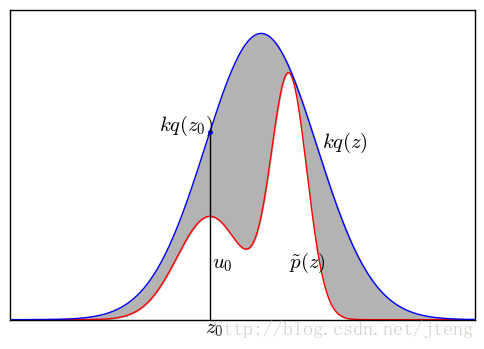
\includegraphics[width=\linewidth]{reject.png}
  \caption{Reject-Sampling Method}
  \label{fig:boat1}
\end{figure}

The basic idea of Reject-Sampling \cite{samp} is to cover the smaller probability distribution with a larger probability distribution. This larger probability distribution $q(x)$ called proposal distribution  and  usually it is a standard distribution such as Uniform distribution, Gaussian distribution, which makes it easier to sample. Then there is a constant $k$ which make $k*q(x) \leq p(x)$.

In each sample process:

\begin{itemize}
  \item Sample a value $x$ from proposal distribution $q(x)$
  \item Get a sample $\mu_0$ from Uniform distribution $[0,k*q(\mu_0)]$.
  \item If $\mu_0 < p(x)$ ,we retain the value otherwise we discard this value. The sampled set is an approximate sample of  distribution.
\end{itemize}

Some cases can be solved  by Reject-Sampling when the probability distribution is not common. However,in the case of high dimensions, Rejection Sampling will encounter two problems. The first is that the proposal  distribution $q$ is difficult to find, and the second is that it is difficult to determine a reasonable value of $k$. These two problems will lead to a high rejection rate and an increase in useless calculations.


\subsection{Markov Chain}
Markov Chain is a random process from state to state in the state space. This process introduce no memory attribute: the probability distribution of the next state can only be determined by the current state, and the events before it in the time series have nothing to do with it. This special type of no memory is called the Markov attribute and as a powerful statistical models Markov chains have many applications in the real world.

At each step of the Markov chain, the system can change from one state to another according to the probability distribution and it also can maintain the current state when it reachs stable state. The change of state is called transition, and the probability associated with different state changes is called transition probability.

In order to obtain a theoretical result, let's look at a smaller example which will facilitate our  calculation demonstration later. Assuming that in a region, people either live in the city or live in the countryside. The matrix below tells us the transition matrix of population migration. For example, the number of the first column  and first row indicates that 90 \% of the population currently living in cities will choose to  live in cities next year and 80 \% of people who live in country will continue to stay in country.
$$
H_x={
\left[ \begin{array}{ccc}
0.9 & 0.1 \\
0.2 & 0.8\\
\end{array}
\right ]}
$$

People assume that nowadays half of the people live in the city and the other half are in the countryside. As a simple start, researchers try to estimate that how much of people will live in city after two years. Analysis shows that 90 \% of people  who currently living in the city will continue to  live in the city after 1 year, and 10\% of people will move to the country. Then another year passed, and 10 \% of those who chose to stay in the city last year moved to the countryside. And 80 \% of those who moved to the village last year will choose to stay in the village. This analysis process is shown  below.
One year later:

$$
H_x=  {
\left[ \begin{array}{ccc}
0.5  & 0.5 \\
\end{array}
\right ]}
\times{
\left[ \begin{array}{ccc}
0.9 & 0.1 \\
0.2 & 0.8\\
\end{array}
\right ]}
=
{
\left[ \begin{array}{ccc}
0.55 & 0.45 \\
\end{array}
\right ]}
$$

One year later:

$$
H_x=  {
\left[ \begin{array}{ccc}
0.55 & 0.45 \\
\end{array}
\right ]}
\times{
\left[ \begin{array}{ccc}
0.9 & 0.1 \\
0.2 & 0.8\\
\end{array}
\right ]}
=
{
\left[ \begin{array}{ccc}
0.585 & 0.415 \\
\end{array}
\right ]}
$$

In fact,it is easy to find that the calculation process above is to do the square of the matrix. As shown in the formula above,on this basis, we can also continue to calculate the situation after $n$ years, that is, the result of calculating the self-multiplication of matrix $A$ n time

The algorithm is as follows:
\begin{itemize}
  \item Enter the Markov chain state transition matrix, set the state transition times threshold,the required number of samples.
  \item Samplfrom any simple probability distribution to get the initial state value.
  \item sample  from the conditional probability distribution and The sample set is the corresponding sample set that meets our stationary distribution.
\end{itemize}

Given the Markov chain state transition matrix corresponding to the stationary distribution of the samples needed to sample, then people can use the Markov chain sampling to obtain the sample set, and then execute Monte Carlo simulation.

But an important question is, given a random distribution at will, how to get the Markov chain state transition matrix $P$ corresponding to it?

\subsection{MCMC  and M-H Sampling}
Mostly, target stationary distribution $\pi(x)$ and a certain Markov chain state transition matrix $Q$ does not satisfy the detailed balance condition:
\[
  \pi(i)Q(i,j) \neq \pi(j)Q(j,i)
\]


a parameter $\alpha(i,j)$ is introduced so that the above formula can take the equal sign.
\[
  \pi(i)Q(i,j)\alpha(i,j) = \pi(j)Q(j,i)\alpha(j,i)
\]

The $\alpha$ can be deducted by symmetry:
\begin{eqnarray*}
\alpha(i,j) &=& \pi(j)Q(j,i)\\
\alpha(j,i) &=& \pi(i)Q(i,j)
\end{eqnarray*}


$\alpha$ is generally called acceptance rate, and the value is between $[0 \sim 1]$, which can be understood as a probability value. This is much like accept-reject sampling, where a common distribution is obtained through a certain acceptance-rejection probability. A common Markov chain with state transition matrix $Q$  can obtain the target sets through a certain acceptance-rejection probability. Obviously the two solutions to the problem are similar\cite{mh}.

MCMC  algorithm is as follows:
\begin{enumerate}
  \item Enter any given Markov chain state transition matrix $Q$, target stable distribution $\pi(x)$, set the threshold of state transition times $n_1$, the number of required samples $n_2$;
  \item Get the initial state value $x_0$ from any simple probability distribution;
  \item For $t$ =0 in $n_1+n_2-1$
    \begin{itemize}
      \item Get the sample value $x_*$ from the conditional probability distribution $Q(x_*|x_0)$.
      \item Sample $U$ from Uniform distribution.
      \item if $u<\pi(x_*)*Q(x_*|x_0)$,then accept $x_*$.
    \end{itemize}
\end{enumerate}


But this sampling algorithm is still more difficult to apply in practice, because in the third step, the accept rate $\alpha$ may be very small, such as 0.1, most of our sampled values ​​are rejected and the sampling efficiency is very low. There is possible that after sampling millions of Markov chains,the result have not yet converged. As a result,the above $n_1$ should be  very large, which is unacceptable.

Metropolis-Hastings sampling also called M-H sampling can solve the problem of low sampling acceptance rate in the previous section.

Expanding both sides of:
\[
  \pi(i)Q(i,j)\alpha(i,j) =  \pi(j)Q(j,i)\alpha(j,i)
\]
At this time the detailed stationary condition is also satisfied. By expanding the equation by $C$ times which can make $c* max(\alpha(i,j)) = 1$ (the maximum expansion of both sides is 1), Metropolis-Hasting sampling significantly improves the acceptance rate.
The transofrmation is:
\[
  \alpha = min(\frac{Q(j,i)\alpha(j,i)}{Q(i,j)\alpha(i,j)},1)
\]

Compare to basic MCMC method, Metropolis Hasting sampling  greatly improves the efficiency of sampling. However, in the era of big data, M-H sampling still faces two major challenges:
\begin{enumerate}

  \item  There are lots of data features and due to the existence of the acceptance rate, the calculation time of M-H sampling required in high dimensions is very considerable, and the algorithm efficiency is very low. At the same time, $ \alpha $ is generally less than 1.  Can it be done without refusing to transfer?

  \item Due to the large feature dimension, it is often difficult to find the joint distribution of each feature dimension of the target, but it is convenient to find the conditional probability distribution between each feature. At this time, is there a  convenient sampling  method in the case of conditional probability distribution between various dimensions?
\end{enumerate}

\subsection{Gibbs Sampling}
Gibbs Sampling Method\cite{bda} is another special MCMC technique used for sampling variales in large dimensions by sampling each variable from its conditional distribution iterative.

Starting from a two-dimensional data distribution, assuming that $\pi(x_1,x_2)$ is a two-dimensional joint data distribution, observe the first two points with the same feature size$A(x_1^{(1)},x_2^{(1)})$ and $B(x_1^{(1)},x_2^{(2))})$.For example:
\[
  \pi(x_1^{(1)},x_2^{(1)})\pi(x_2^{(2)}|x_1^{(1)}) = \pi(x_1^{(1)})\pi(x_2^{(2)}|x_1^{(1)})\pi(x_2^{(1)}|x_1^{(1)})
\]

\[
  \pi(x_1^{(1)},x_2^{(1)})\pi(x_2^{(1)}|x_1^{(1)}) = \pi(x_1^{(1)})\pi(x_2^{(2)}|x_1^{(1)})\pi(x_2^{(1)}|x_1^{(1)})
\]

Since the right sides of the two formulas are equal, we have:
\[
  \pi(x_1^{(1)},x_2^{(1)})\pi(x_2^{(2)}|x_1^{(1)}) =   \pi(x_1^{(1)},x_2^{(1)})\pi(x_2^{(1)}|x_1^{(1)})
\]

Observing the above detail balance formula , it shows that on the straight line of $x_1 = x_1^{(1)}$, if the conditional probability distribution $\pi(x_2|x_1^{(1)})$ is used as the state transition probability of the Markov chain, the transition between any two points meets Detail balance conditions! In the same way, on the straight line of $x_2 = x_2^{(1)}$, if the conditional probability distribution $\pi(x_1|x_2^{(1)})$  is used as the state transition probability of the Markov chain, the transition between any two points also meets the detail balance condition.


With the  transition matrix and conditional probability, a two-dimensional Gibbs sample can be applied to get samples conventiently.
The algorithm is as follows:
\begin{enumerate}
  \item Given stationary distribution $\pi(x_1,x_2)$,Set the threshold value of the number of state transitions $n_1$, the number of required samples $n_2$.
  \item Randomly initialize values $x_1^{(1)}$ and $x_2^{(1)}$.
  \item for t in [0,n1+n2-1]:
      \begin{itemize}
        \item Get sample $x_2^{(t+1)}$ from conditional distribution $p(x_2|x_1^t)$
        \item Get sample $x_1^{(t+1)}$ from conditional distribution $p(x_1|x_2^t)$
      \end{itemize}
\end{enumerate}
